% !TEX program = pdflatex
% !TEX options = -synctex=1 -interaction=nonstopmode -file-line-error "%DOC%"
% 作业模板
\documentclass[UTF8,10pt,a4paper]{article}
\usepackage{ctex}
\newfontfamily\menlo{MONACO.TTF}
\usepackage{amsmath}
\usepackage{diagbox}
\usepackage{float}
\usepackage{listings}
\usepackage{multirow}
\usepackage{tabularx}

\usepackage{url}
\usepackage{xcolor}
\newcommand{\tabincell}[2]{\begin{tabular}{@{}#1@{}}#2\end{tabular}}

\lstset{
    breaklines,                                 % 自动将长的代码行换行排版
    extendedchars=false,                        % 解决代码跨页时,章节标题,页眉等汉字不显示的问题
    backgroundcolor=\color[rgb]{0.96,0.96,0.96},% 背景颜色
    keywordstyle=\color{blue}\bfseries,         % 关键字颜色
    identifierstyle=\color{black},              % 普通标识符颜色
    commentstyle=\color[rgb]{0,0.6,0},          % 注释颜色
    stringstyle=\color[rgb]{0.58,0,0.82},       % 字符串颜色
    showstringspaces=false,                     % 不显示字符串内的空格
    numbers=left,                               % 显示行号
    numberstyle=\tiny\menlo,                    % 设置数字字体
    basicstyle=\small\menlo,                    % 设置基本字体
    captionpos=t,                               % title在上方(在bottom即为b)
    frame=single,                               % 设置代码框形式
    rulecolor=\color[rgb]{0.8,0.8,0.8},         % 设置代码框颜色
}  

\usepackage{pythonhighlight}
\usepackage{listings}
\usepackage{xcolor}
\usepackage{graphicx}
\usepackage[a4paper,left=2cm,right=2cm,top=2cm,bottom=2cm]{geometry}
\usepackage{fancyhdr}
% \catcode`\。=\active
% \newcommand{。}{.}
\newcommand{\CourseName}{操作系统(Operating System)}
\newcommand{\CourseCode}{CS307 \& CS356}
\newcommand{\Semester}{2020-2021学年第二学期}
\newcommand{\ProjectName} {\Huge{Project 6}} 
\newcommand{\StudentName}{刘涵之}
\newcommand{\StudentID}{519021910102}
\usepackage[vmargin=1in,hmargin=.5in]{geometry}
\usepackage{fancyhdr}
\usepackage{lastpage}
\usepackage{calc}
\pagestyle{fancy}
\fancyhf{}
\fancyhead[L]{\CourseName}
\fancyhead[C]{\ProjectName}
\fancyhead[R]{\StudentName}
\fancyfoot[R]{\thepage\ / \pageref{LastPage}}
\setlength\headheight{12pt}
\fancypagestyle{FirstPageStyle}{
    \fancyhf{}
    \fancyhead[L]{\CourseName\\
        \CourseCode\\
        \Semester}
    \fancyhead[C]{\large\bfseries\ProjectName \\}
    \fancyhead[R]{Name: \makebox[\widthof{\StudentID}][s]{\StudentName}\\
        ID : \StudentID\\
        }
    \fancyfoot[R]{\thepage\ / \pageref{LastPage}}
    \setlength\headheight{36pt}
}
\usepackage{amsmath,amssymb,amsthm,bm}
\allowdisplaybreaks[4]
\newtheoremstyle{Problem}
{}
{}
{}
{}
{\bfseries}
{.}
{ }
{第\thmnumber{ #2}\thmname{ #1}\thmnote{ (#3)} 得分: \underline{\qquad\qquad}}
\theoremstyle{Problem}
\newtheorem{prob}{题}
\newtheoremstyle{Solution}
{}
{}
{}
{}
{\bfseries}
{:}
{ }
{\thmname{#1}}
\makeatletter
\def\@endtheorem{\qed\endtrivlist\@endpefalse}
\makeatother
\theoremstyle{Solution}
\newtheorem*{sol}{解}
\title{Project 6: Banker's Algorithm}
\date{}
% \usepackage{graphicx}
\begin{document}
\maketitle
\thispagestyle{FirstPageStyle}

For this project, you will write a program that implements the banker’s algorithm discussed in Section 8.6.3. Customers request and release resources from the bank. The banker will grant a request only if it leaves the system in a safe state. A request that leaves the system in an unsafe state will be denied. Although the code examples that describe this project are illustrated in C, you may also develop a solution using Java.

The banker will grant a request if it satisfies the safety algorithm outlined in Section 8.6.3.1. If a request does not leave the system in a safe state, the banker will deny it. Function prototypes for requesting and releasing resources are as follows:

\begin{lstlisting}[language = c]
int request_resources(int target, int req[]);
void release_resources(int target, int release[]);
\end{lstlisting}

The \textbf{request\_resources()} function should return 0 if successful and –1 if
unsuccessful.

Your program will initially read in a file containing the maximum number of requests for each customer. Your program will then have the user enter commands responding to a request of resources, a release of resources, or the current values of the different data structures. Use the command ‘\textbf{RQ}’ for requesting resources, ‘\textbf{RL}’ for releasing resources, and ‘\textbf{*}’ to output the values of the different data structures.

\textbf{Design:} My design for this task is shown as follows:

\begin{itemize}
    \item I use four arrays to track the current state: \texttt{available}, \texttt{maximum}, \texttt{allocation}, \texttt{need}. 
    
    \item The content of \texttt{maximum} will be initialized from the file \texttt{max}.
    
    \item \textbf{check\_safe()} function will use the banker algorithm to check the current state.
    
    \item \textbf{output()} function will output the current state.
    
    \item When requesting resources, changes will be done if and only if it passes \textbf{check\_safe()} function.
    
    \item When releasing resources, changes will be done immediately.
\end{itemize}

The code of \texttt{banker.c} is shown as follows.

\begin{lstlisting}[language = c]
#include <stdio.h>
#include <stdlib.h>
#include <unistd.h>
#include <string.h>

#define NUMBER_OF_CUSTOMERS 5
#define NUMBER_OF_RESOURCES 4

/* the available amount of each resource */
int available[NUMBER_OF_RESOURCES];
/*the maximum demand of each customer */
int maximum[NUMBER_OF_CUSTOMERS][NUMBER_OF_RESOURCES];
/* the amount currently allocated to each customer */
int allocation[NUMBER_OF_CUSTOMERS][NUMBER_OF_RESOURCES];
/* the remaining need of each customer */
int need[NUMBER_OF_CUSTOMERS][NUMBER_OF_RESOURCES];

int check_safe();
int request_resources(int target, int req[]);
void release_resources(int target, int release[]);

int request_resources(int target, int req[]) {
    for (int i = 0; i < NUMBER_OF_RESOURCES; i++){
        if (req[i] < 0) {
            fprintf(stdout, "[Error] Request less than 0! \n");
            return 1;
        }
        if (req[i] > need[target][i]) {
            fprintf(stdout, "[Error] Request more than need! \n");
            return 1;
        }
    }
            
    for (int i = 0; i < NUMBER_OF_RESOURCES; i++){
        available[i] -= req[i];
        allocation[target][i] += req[i];
        need[target][i] = maximum[target][i] - allocation[target][i];
    }

    if (check_safe() == 1) {
        // unsafe, rollback
        for (int i = 0; i < NUMBER_OF_RESOURCES; i++){
            available[i] += req[i];
            allocation[target][i] -= req[i];
            need[target][i] = maximum[target][i] - allocation[target][i];
        }
        fprintf(stdout, "[Unsafe] Denied. \n");
        return 1;
    } else {
        fprintf(stdout, "[Safe] Accepted. \n");
        return 0;
    }
}

void release_resources(int target, int release[]){
    for (int i = 0; i < NUMBER_OF_RESOURCES; i++){
        if (release[i] < 0) {
            fprintf(stdout, "[Error] Release less than 0! \n");
            return;
        }
        if (release[i] > allocation[target][i]) {
            fprintf(stdout, "[Error] Release more than allocated! \n");
            return;
        }
    }
    
    for (int i = 0; i < NUMBER_OF_RESOURCES; i++){
        available[i] += release[i];
        allocation[target][i] -= release[i];
        need[target][i] = maximum[target][i] - allocation[target][i];
    }
    fprintf(stdout, "[Safe] Accepted. \n");
    return;
}

int initialize(int argc, char *argv[]) {
    for (int i = 0; i < NUMBER_OF_RESOURCES; i++)
        available[i] = atoi(argv[i]);

    FILE *stream = fopen("max", "r");
    for (int i = 0; i < NUMBER_OF_CUSTOMERS; i++) {
        fscanf(stream, "%d", &maximum[i][0]);
        for (int j = 1; j < NUMBER_OF_RESOURCES; j++) {
            fscanf(stream, ",%d", &maximum[i][j]);
        }
    }
    fclose(stream);

    for (int i = 0; i < NUMBER_OF_CUSTOMERS; i++)
        for (int j = 0; j < NUMBER_OF_RESOURCES; j++) {
            need[i][j] = maximum[i][j];
            allocation[i][j] = 0;
        }
    return 0;
}

int check_safe() {
    int used[NUMBER_OF_CUSTOMERS];
    int available_[NUMBER_OF_RESOURCES];

    for (int i = 0; i < NUMBER_OF_RESOURCES; i++)
        available_[i] = available[i];

    for (int i = 0; i < NUMBER_OF_CUSTOMERS; i++)
        used[i] = 0;
    
    for (int i = 0; i < NUMBER_OF_CUSTOMERS; i++) {
        // find a customer to use
        int safe = 0;
        for (int j = 0; j < NUMBER_OF_CUSTOMERS; j++) {
            if (used[j] == 0) {
                int can = 1;
                for (int res = 0; res < NUMBER_OF_RESOURCES; res ++) {
                    if (need[j][res] > available_[res]) {
                        can = 0;
                        break;
                    }
                }
                if (can == 1) {
                    used[j] = 1;
                    safe = 1; // customer j can be satisfied!
                    for (int res = 0; res < NUMBER_OF_RESOURCES; res ++) {
                        available_[res] += allocation[j][res];
                    }
                    break;
                }
            }
        }
        if (safe == 0) {
            return 1;
        }
    }
    return 0;
}

void output() {
    fprintf(stdout, "#####     Current State     #####\n");
    fprintf(stdout, "  Available: [ ");
    for (int i = 0; i < NUMBER_OF_RESOURCES - 1; i++)
        fprintf(stdout, "%d , ", available[i]);
    fprintf(stdout, "%d ]\n", available[NUMBER_OF_RESOURCES - 1]);

    fprintf(stdout, "  Maximum: ");
    for (int i = 0; i < NUMBER_OF_CUSTOMERS; i++) {
        if (i != 0) fprintf(stdout, "           ");
        fprintf(stdout, "[ ");
        for (int j = 0; j < NUMBER_OF_RESOURCES - 1; j++) {
            fprintf(stdout, "%d , ", maximum[i][j]);
        }
        fprintf(stdout, "%d ]\n", maximum[i][NUMBER_OF_RESOURCES - 1]);
    }

    fprintf(stdout, "  Allocation: ");
    for (int i = 0; i < NUMBER_OF_CUSTOMERS; i++) {
        if (i != 0) fprintf(stdout, "              ");
        fprintf(stdout, "[ ");
        for (int j = 0; j < NUMBER_OF_RESOURCES - 1; j++) {
            fprintf(stdout, "%d , ", allocation[i][j]);
        }
        fprintf(stdout, "%d ]\n", allocation[i][NUMBER_OF_RESOURCES - 1]);
    }

    fprintf(stdout, "  Need: ");
    for (int i = 0; i < NUMBER_OF_CUSTOMERS; i++) {
        if (i != 0) fprintf(stdout, "        ");
        fprintf(stdout, "[ ");
        for (int j = 0; j < NUMBER_OF_RESOURCES - 1; j++) {
            fprintf(stdout, "%d , ", need[i][j]);
        }
        fprintf(stdout, "%d ]\n", need[i][NUMBER_OF_RESOURCES - 1]);
    }
}

int main(int argc, char *argv[]) {
    if (argc != NUMBER_OF_RESOURCES + 1) {
        fprintf(stdout, "[Error] Wrong input. \n");
        exit(1);
    }
    initialize(argc, argv + 1);
    if (check_safe() == 1) {
        fprintf(stdout, "[Error] Unsafe initial state. \n");
        exit(1);
    }

    while (1) {
        char s1[100];
        fprintf(stdout, "Banker>>");
        fscanf(stdin, "%s", s1);
        if (strcmp(s1, "*") == 0) {
            output();
            continue;
        } else
        if (strcmp(s1, "RQ") == 0) {
            int target;
            fscanf(stdin, "%d", &target);

            int req[NUMBER_OF_RESOURCES];
            for (int i = 0; i < NUMBER_OF_RESOURCES; i++){
                fscanf(stdin, "%d", &req[i]);
            }

            request_resources(target, req);
        } else
        if (strcmp(s1, "RL") == 0) {
            int target;
            fscanf(stdin, "%d", &target);

            int req[NUMBER_OF_RESOURCES];
            for (int i = 0; i < NUMBER_OF_RESOURCES; i++){
                fscanf(stdin, "%d", &req[i]);
            }

            release_resources(target, req);
        } else {
            fprintf(stdout, "[Error] Unexpected input! \n");
        }
    }
    output();
}
\end{lstlisting}





Makefile for this task is shown as follow.
\begin{lstlisting}
CC=gcc
CFLAGS=-Wall

all: banker.o
	$(CC) $(CFLAGS) -o banker banker.o

banker.o: banker.c
	$(CC) $(CFLAGS) -c banker.c

clean:
	rm -rf *.o
	rm -rf banker
\end{lstlisting}

The \texttt{max} file used here is:

\begin{lstlisting}
6,4,7,3
4,2,3,2
2,5,3,3
6,3,3,2
5,6,7,5
\end{lstlisting}


The execution result is shown as follow. All functions mentioned above have been tested successfully. 

\begin{figure}[H]
    \centering
    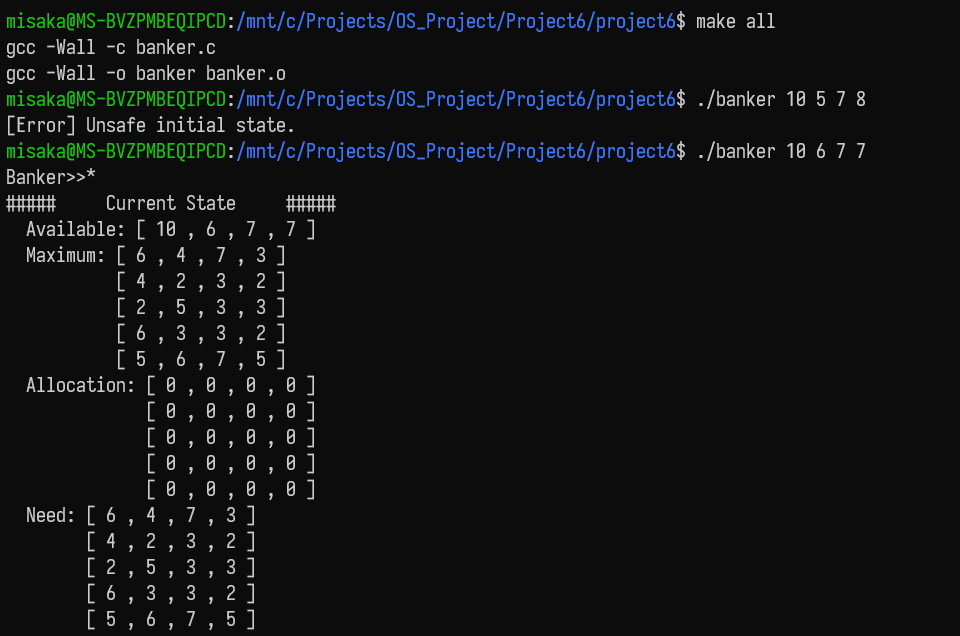
\includegraphics[width=400pt]{1.png}
    \caption{Banker's Algorithm}
    \label{3}
\end{figure}

\begin{figure}[H]
    \centering
    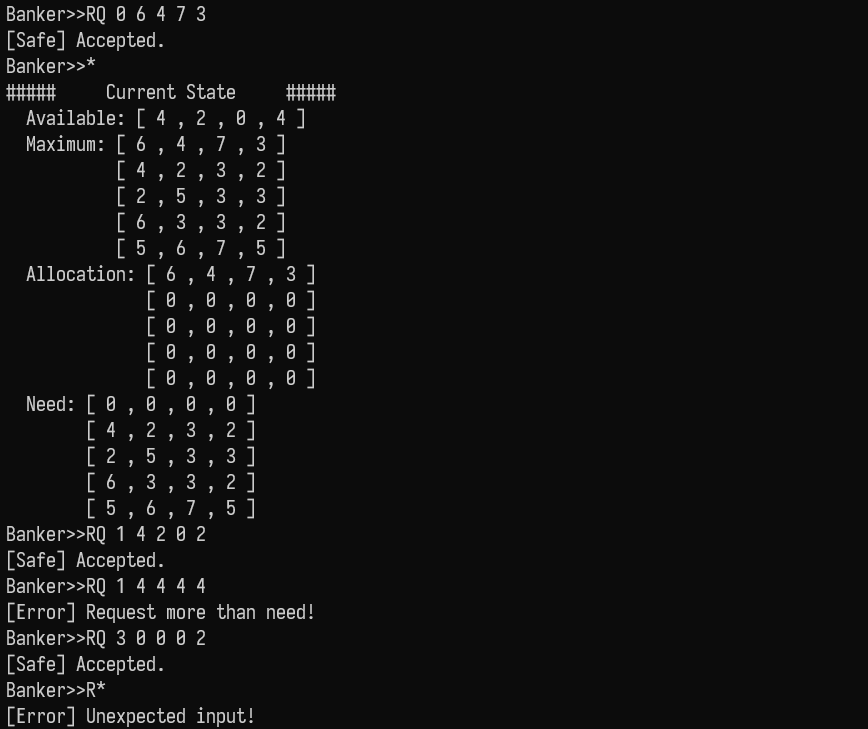
\includegraphics[width=400pt]{2.png}
    \caption{Banker's Algorithm}
    \label{3}
\end{figure}

\begin{figure}[H]
    \centering
    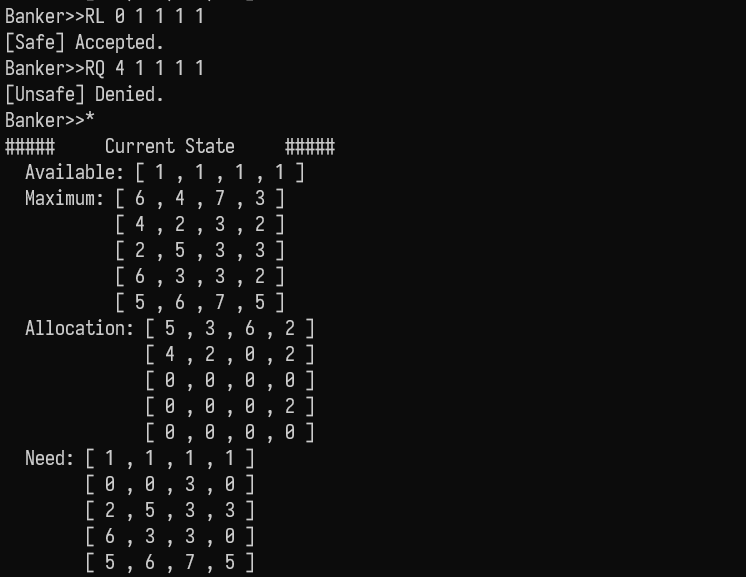
\includegraphics[width=400pt]{3.png}
    \caption{Banker's Algorithm}
    \label{3}
\end{figure}

\end{document}